\section{Conclusion}
\author{Kévin Moreau}


\begin{frame}
	\frametitle{Rappel du contexte}

	\begin{block}{L'entreprise Dynamease}
	 \begin{itemize}
      \item Start-up ;
	  \item Service de mise en communication contextualisée.
	 \end{itemize}
	\end{block}

    \begin{center}
	  \begin{figure}
        \includegraphics[scale=0.30]{images/dynamease.pdf}
	   \caption{Communication contextualisé}
	  \end{figure}
	\end{center}
\end{frame}

\begin{frame}
	\frametitle{Rappel du contexte}
	
	\begin{center}
	  \begin{figure}
	   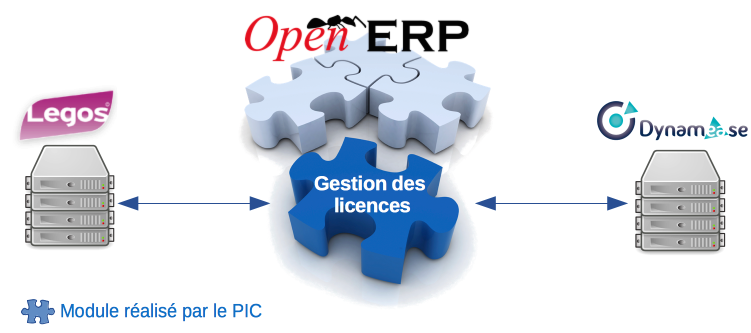
\includegraphics[width=0.80\textwidth]{images/schemaGlobal.png}
	   \caption{Schéma d'intégration du projet}
	  \end{figure}
	\end{center}

    \begin{block}{Le PIC Dynamease}
	 \begin{itemize}
	  \item Gestion de la vente des licences client :
      \item Gestion de la comptabilité associée
	  \item Liaison avec le fournisseur de numéros téléphoniques.
	 \end{itemize}
	\end{block}

\end{frame}


